\documentclass[a4paper,12pt]{article}
\usepackage{polyglossia}
\setdefaultlanguage{russian}
\usepackage{fontspec}
\setmainfont{Times New Roman}
\newfontfamily\cyrillicfont{Times New Roman}
\newfontfamily\cyrillicfonttt{FreeMono}
\usepackage{graphicx}
\usepackage{amsmath, amssymb}
\usepackage{hyperref}
\usepackage{float}
\usepackage{listings}
\usepackage{caption}
\usepackage{geometry}
\usepackage{xcolor}
\geometry{left=2cm,right=2cm,top=2cm,bottom=2cm}
\hypersetup{pdfborder=0 0 0}
\headsep=8mm
\footskip=20mm
\hypersetup{pdfstartview=FitH, linkcolor=linkcolor, urlcolor=urlcolor, colorlinks=true}

\definecolor{strings}{rgb}{0,0.6,0}
\definecolor{comments}{rgb}{0,0.3,0}
\definecolor{numbers}{rgb}{0.5,0.5,0.5}
\definecolor{keywords}{rgb}{0.09,0.61,0.95}
\definecolor{background}{rgb}{0.97,0.97,0.97}
\hypersetup{
    colorlinks=true,
    linkcolor=blue,
    filecolor=magenta,      
    urlcolor=cyan,
    pdftitle={Overleaf Example},
    pdfpagemode=FullScreen,
    }

\lstdefinestyle{codestyle}{
    backgroundcolor=\color{background},
    commentstyle=\color{comments},
    keywordstyle=\color{keywords},
    stringstyle=\color{strings},
    numberstyle=\tiny\color{numbers},
    basicstyle=\ttfamily\scriptsize,
    breakatwhitespace=false,
    breaklines=true,
    captionpos=b,
    inputencoding=utf8,
    keepspaces=false,
    numbers=left,
    numbersep=5pt,
    showspaces=false,
    showstringspaces=false,
    showtabs=false,
    tabsize=2,
    extendedchars=true
}

\lstset{style=codestyle}

\begin{document}    

\begin{titlepage}
    \centering
    {\large Федеральное государственное автономное образовательное учреждение\par}
    {\large высшего образования\par}
    {\bfseries САНКТ-ПЕТЕРБУРГСКИЙ НАЦИОНАЛЬНЫЙ ИССЛЕДОВАТЕЛЬСКИЙ УНИВЕРСИТЕТ ИТМО\par}
    {\bfseries Факультет систем управления и робототехники\par}
    \vfill
    {\Large \bfseries Лабораторная работа №6\par}
    {\Large \bfseries Морфологический анализ изображений\par}
    \vfill
    
    \begin{flushright}
        Студенты: Бахтаиров Р.А.,\\ 
        Сайфуллин Д.Р. \\
        Поток: Тех.Зр R23 1.1 \\
        Преподаватель: Шаветов С.В.
    \end{flushright}
    \vfill
    Санкт-Петербург\\
    2025 г.
\end{titlepage}

\tableofcontents
\newpage

\section{Цель работы}
Освоение принципов математической морфологии в области об-
работки и анализа изображений.

\section{Теория}
Математическая морфология — раздел прикладной математики и теории обработки изображений, основанный на анализе формы и структуры объектов с помощью линейно-сдвиговых преобразований множества пикселей. Морфологический подход рассматривает изображение \(A\) как множество точек в дискретном пространстве, а структурный элемент \(B\) — как небольшое «окно» для анализа локальной геометрии изображения.

Основные операции бинарной морфологии над множеством \(A\) и структурным элементом \(B\):
\begin{itemize}
  \item \textbf{Дилатация} (расширение): 
    \[
      A \oplus B = \{\,z \mid (B)_z \cap A \neq \varnothing \,\},
    \]
  \item \textbf{Эрозия} (сжатие):
    \[
      A \ominus B = \{\,z \mid (B)_z \subseteq A \,\},
    \]
  \item \textbf{Открытие} (удаление мелких объектов и шумов): 
    \[
      A \circ B = (A \ominus B) \oplus B,
    \]
  \item \textbf{Замыкание} (заполнение «дырок» и соединение близких объектов):
    \[
      A \bullet B = (A \oplus B) \ominus B,
    \]
\end{itemize}

Дополнительные производные операции:
\begin{itemize}
  \item \textbf{Морфологический градиент} 
    \(\;\mathrm{grad}(A,B) = (A \oplus B) - (A \ominus B)\), 
    служит для выделения контура объекта.
  \item \textbf{Top-hat} 
    \(\;\mathrm{tophat}(A,B) = A - (A \circ B)\), 
    позволяет извлечь «светлые» мелкие детали.
  \item \textbf{Black-hat} 
    \(\;\mathrm{blackhat}(A,B) = (A \bullet B) - A\), 
    выявляет «тёмные» мелкие дефекты на фоне.
  \item \textbf{Hit-or-miss} — структурно-селективная операция поиска заданных шаблонов.
\end{itemize}

Структурный элемент \(B\) может иметь форму прямоугольника, креста или эллипса.

Основные области применения математической морфологии:
\begin{itemize}
  \item Фильтрация шумов и удаления мелких артефактов на бинарных изображениях.
  \item Сегментация и разделение перекрывающихся объектов (в том числе методом водораздела).
  \item Выделение контуров и структурных элементов формы.
  \item Поиск связных компонентов и анализ их статистических характеристик (площадь, границы, центр масс).
\end{itemize}

\section{Базовые морфологические операции}
В этой задаче необходимо выбрать произвольное бинарное с дефектами формы и применить к нему основные морфологические операции для удаления или минимизации этих дефектов.

\begin{figure}[H]
    \centering
    
\includegraphics[width=0.4\textwidth]{images/gosu2.png}
    \caption{Исходное изображение с внешними выступами и внутренними «дырами».}
\end{figure}

На рисунке видны выбоины внутри объектов и мелкие выступы по контуру.
Преобразуем изображение в отенки серого:

\begin{figure}[H]
    \centering
    
\includegraphics[width=0.4\textwidth]{result/1_grayscale.png}
    \caption{Исходное изображение в серых тонах.}
\end{figure}
  
Чтобы избавиться от мелких «дыр» внутри объектов, к изображению применим операцию удаления компонентов меньших 70 пикселей (\texttt{bwareaopen}), после чего результат инвертирован обратно.

\begin{figure}[H]
    \centering
    
\includegraphics[width=0.4\textwidth]{result/1_beware_inside.png}
    \caption{Исходное изображение после \texttt{bwareaopen}.}
\end{figure}

Эллиптическим структурным элементом \(3\times3\) с двумя итерациями эрозии были «стёрты» тонкие выступающие фрагменты, отделив их от крупных областей.

\begin{figure}[H]
    \centering
    
\includegraphics[width=0.4\textwidth]{result/1_erosion.png}
    \caption{Исходное изображение после эрозии краёв.}
\end{figure}

На полученном после эрозии изображении снова применим операцию удаления компонентов меньших 140 пикселей. Это позволит окончательно избавиться от отдельных «висящих» линий.

\begin{figure}[H]
    \centering
    
\includegraphics[width=0.4\textwidth]{result/1_beware_out.png}
    \caption{Исходное изображение после \texttt{bwareaopen}.}
\end{figure}

Чтобы компенсировать усадку от эрозии, проведем дилатацию тем же элементом с двумя итерациями — объекты распухли к исходным размерам.

\begin{figure}[H]
    \centering
    
\includegraphics[width=0.4\textwidth]{result/1_dilation.png}
    \caption{Исходное изображение после дилатации.}
\end{figure}

Далее три итерации операции замыкания закрыли узкие щели и разрывы, которые не удалось устранить предыдущими шагами.

\begin{figure}[H]
    \centering
    
\includegraphics[width=0.4\textwidth]{result/1_close.png}
    \caption{Исходное изображение после замыкания.}
\end{figure}

Для удаления оставшихся мелких шумов применим ещё один цикл \texttt{bwareaopen} (порог 80 пикселей) к инвертированному результату замыкания.

\begin{figure}[H]
    \centering
    
\includegraphics[width=0.4\textwidth]{result/1_beware_inside_2.png}
    \caption{Итог после всех этапов очистки.}
\end{figure}

Полученная последовательность операций обеспечивает:
\begin{itemize}
  \item Надёжное удаление внутренних шумов без существенного искажения крупных объектов.
  \item Эффективное отделение мелких выступов через сочетание эрозии и удаления малых компонентов.
  \item Восстановление размеров объектов с помощью дилатации и замыкания, что сохраняет исходную форму.
\end{itemize}

\section{Разделение объектов}
В этой задаче мы разделили объекты на изображении с наложенными друг на друга элементами с помощью сочетания пороговой бинаризации и последовательных морфологических операций. Изображение с которым будем работать и его grayscale:

\begin{figure}[H]
    \centering
    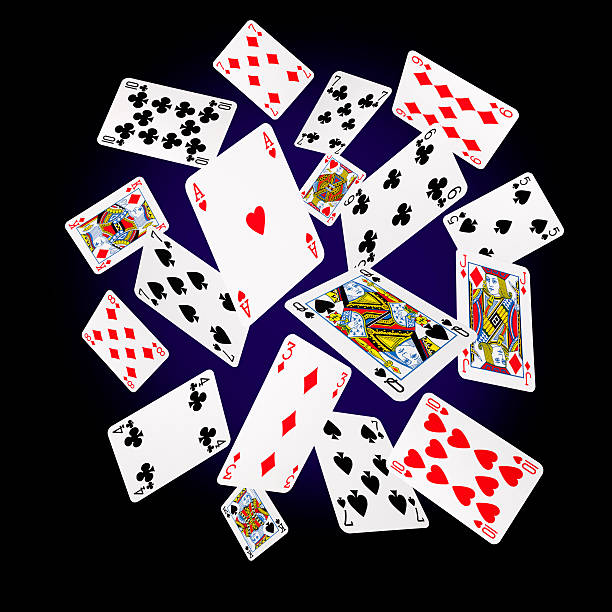
\includegraphics[width=0.4\textwidth]{images/cards2.jpg}
    \caption{Исходное изображение.}
\end{figure}
\begin{figure}[H]
    \centering
    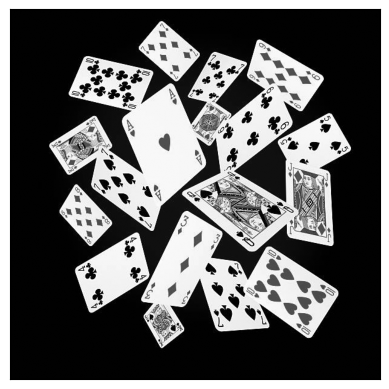
\includegraphics[width=0.4\textwidth]{result/2_grayscale.png}
    \caption{Исходное изображение в серых тонах.}
\end{figure}

Применим биноризацию с порогом 50 и \texttt{bwareaopen} с порогом 400, чтобы выделить карты на фоне. 

\begin{figure}[H]
    \centering
    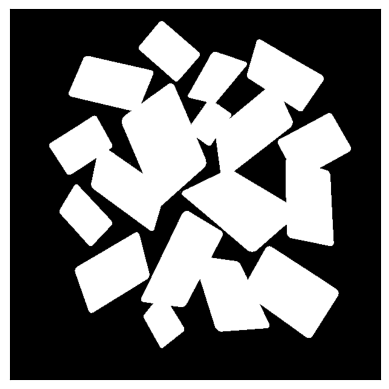
\includegraphics[width=0.4\textwidth]{result/2_bin.png}
    \caption{Изображение после бинаризации.}
\end{figure}

В результате мы получили бинарное изображение, где карты выделены белым цветом, а фон — чёрным. Для надёжного определения центральных областей карт мы выполним трёхкратную эрозию эллиптическим элементом \(10\times10\) и затем шестикратную эрозию прямоугольным \(3\times3\). 

\begin{figure}[H]
    \centering
    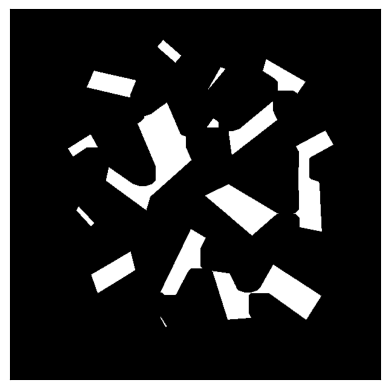
\includegraphics[width=0.4\textwidth]{result/2_erosion.png}
    \caption{Изображение после эрозии.}
\end{figure}
\begin{figure}[H]
    \centering
    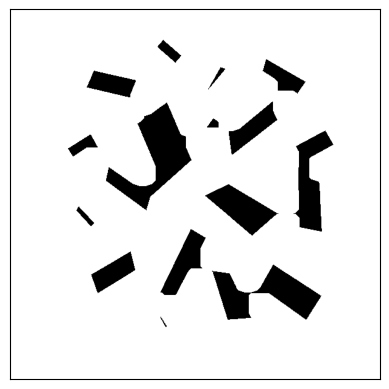
\includegraphics[width=0.4\textwidth]{result/2_erosion_invert.png}
    \caption{Инверсия изображения после эрозии.}
\end{figure}

Инверсия этой маски дала первую приблизительную карту границ между объектами. Теперь мы можем последовательно «срезать» границу эрозией и удалить открытием, аккумулируя разницу на каждом шаге.

\begin{figure}[H]
    \centering
    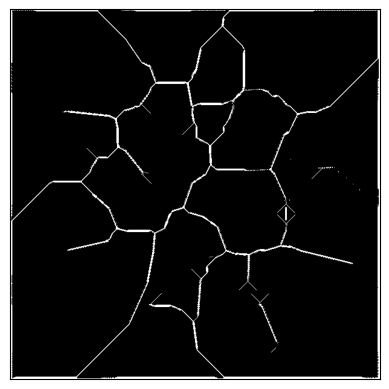
\includegraphics[width=0.4\textwidth]{result/2_borders.png}
    \caption{Изображение с линиями разделения.}
\end{figure}

В результате получилась тонкая маска разделителей, чётко проходящая между картами.

\begin{figure}[H]
    \centering
    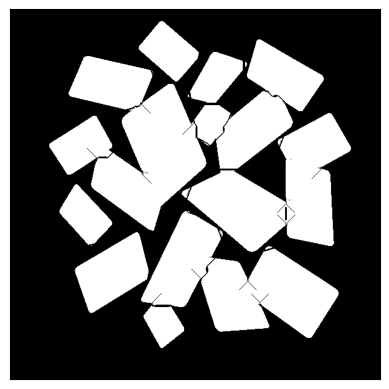
\includegraphics[width=0.4\textwidth]{result/2_split.png}
    \caption{Изображение с линиями разделения.}
\end{figure}

На рисунке показано, как маска исходных карт очищена от разделителей. Применим ее к исходному изображению:

\begin{figure}[H]
    \centering
    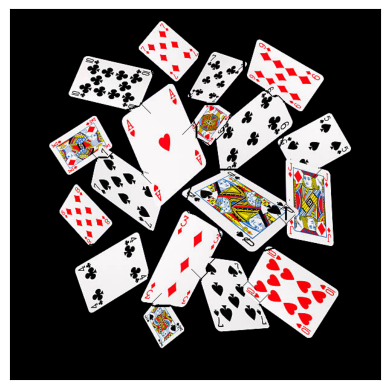
\includegraphics[width=0.4\textwidth]{result/2_split_color.png}
    \caption{Финальный результат.}
\end{figure}

Мы видим как на исходном цветном изображении, в котором линии разделения обнулили пиксели- разделители, отделили карты друг от друга.

Можем сделать выводы:
\begin{itemize}
    \item Комбинация «грубых» (большой элемент + многократная эрозия) и «тонких» (малый элемент + итеративное открытие) морфологических операций позволила чётко выделить центральные области и аккуратно вырезать узкие разделители.
    \item Маска разделителей оказалась достаточно тонкой, чтобы не нарушать форму карт, при этом полностью разрывая перекрытие.
    \item Финальное применение побитовой операции к исходному цветному изображению показало эффективность метода: все пункты наложения карт были успешно разъединены.
\end{itemize} 

\section{Сегментация}
В этой задаче необходимо разделить перекрывающиеся круглые объекты на изображении методом управляемого водораздела. Последовательность шагов включает бинаризацию и очистку, выделение маркеров, построение объединённой карты маркеров и собственно запуск алгоритма \texttt{watershed}. 

Изображение с которым будем работать и его преобразования:

\begin{figure}[H]
    \centering
    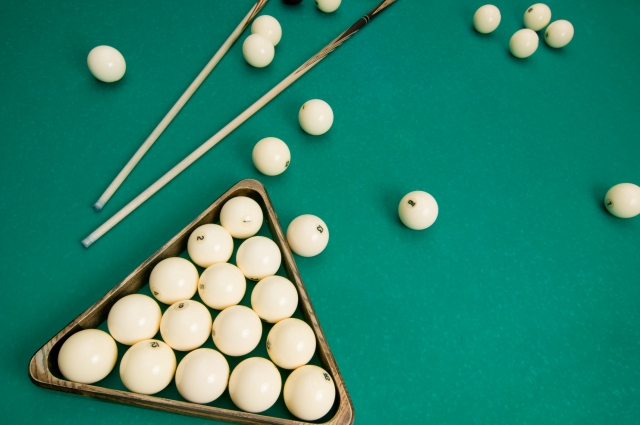
\includegraphics[width=0.4\textwidth]{images/balls.jpg}
    \caption{Исходное изображение.}
\end{figure}
\begin{figure}[H]
    \centering
    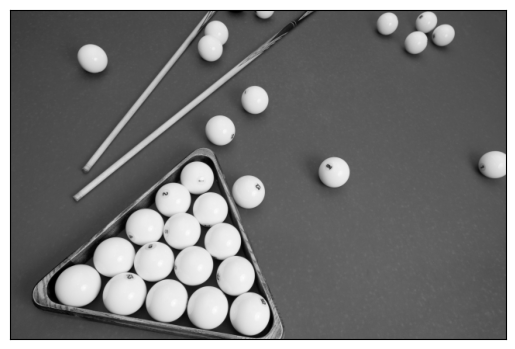
\includegraphics[width=0.4\textwidth]{result/3_grayscale.png}
    \caption{Исходное изображение в серых тонах.}
\end{figure}
\begin{figure}[H]
    \centering
    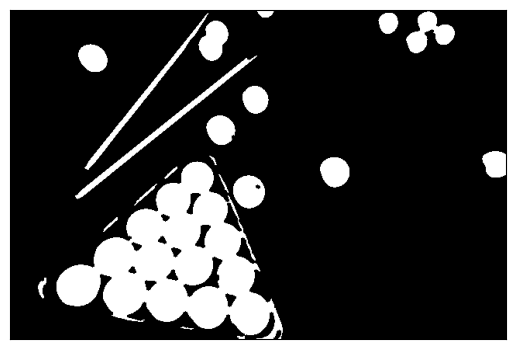
\includegraphics[width=0.4\textwidth]{result/3_bw_clean.png}
    \caption{Бинаризация + удаление мелких шумов.}
\end{figure}

На рисунке показан результат автоматической бинаризации, после чего с помощью двух операций \texttt{bwareaopen} (порог 20\,px) и одного замыкания (структурный элемент \(5\times5\)) были удалены внутренние дефекты и сглажены контуры.

\begin{figure}[H]
    \centering
    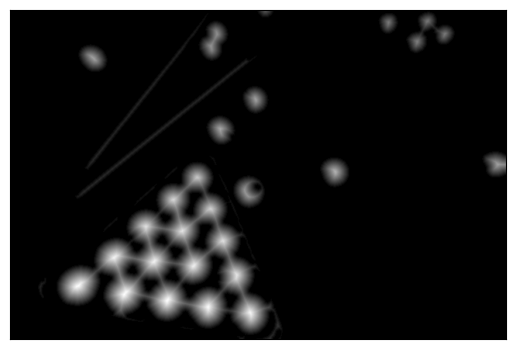
\includegraphics[width=0.4\textwidth]{result/3_distance.png}
    \caption{Карта расстояний.}
\end{figure}
\begin{figure}[H]
    \centering
    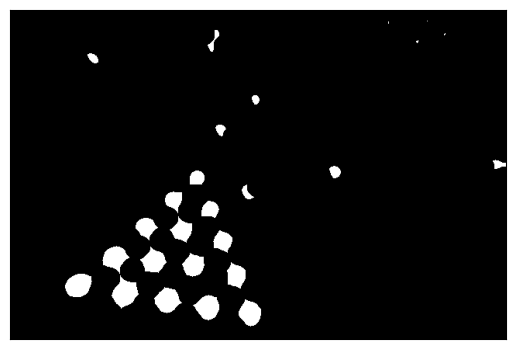
\includegraphics[width=0.4\textwidth]{result/3_fg.png}
    \caption{Максимумы для переднего плана.}
\end{figure}

На карте расстояний локальные «блики» соответствуют центрам шаров. Порогирование при 0.46 * максимального значения даёт надёжную маску — маркеры переднего плана.

\begin{figure}[H]
    \centering
    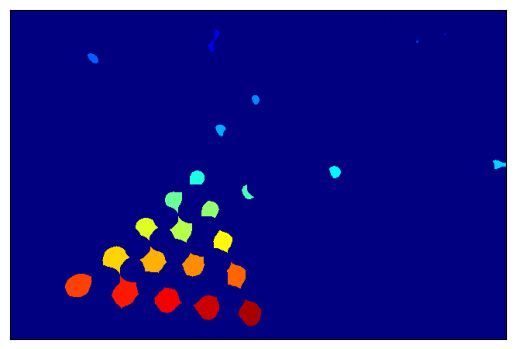
\includegraphics[width=0.4\textwidth]{result/3_fg_markers.png}
    \caption{Маркеры переднего плана.}
\end{figure}
\begin{figure}[H]
    \centering
    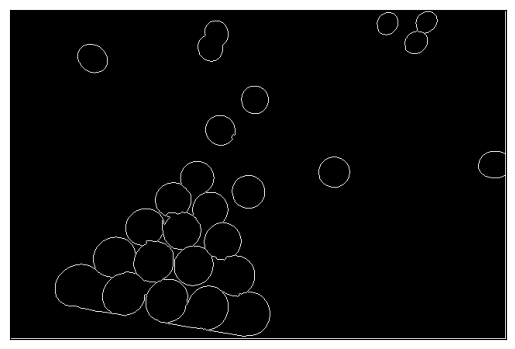
\includegraphics[width=0.4\textwidth]{result/3_bg.png}
    \caption{Маска заднего плана.}
\end{figure}
\begin{figure}[H]
    \centering
    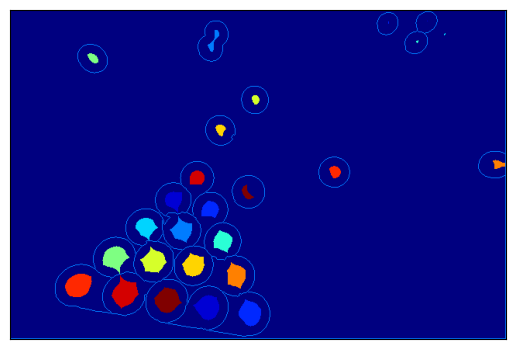
\includegraphics[width=0.4\textwidth]{result/3_all_markers.png}
    \caption{Объединённая карта маркеров.}
\end{figure}

Фоновые маркеры извлекаются по контуру областей, помеченным алгоритмом \texttt{watershed} на предварительном проходе. Объединив передний план и задний план, мы получаем полную карту маркеров, которую подаём на второй запуск \texttt{watershed}.

\begin{figure}[H]
    \centering
    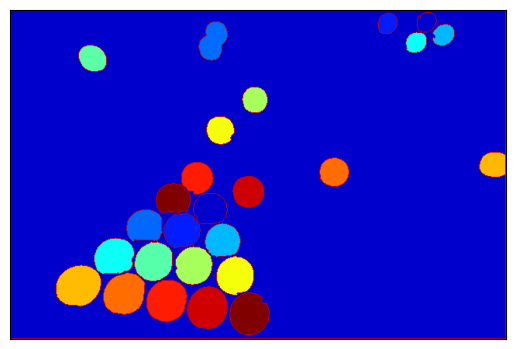
\includegraphics[width=0.4\textwidth]{result/3_watershed_markers.png}
    \caption{Маркеры после водораздела.}
\end{figure}
\begin{figure}[H]
    \centering
    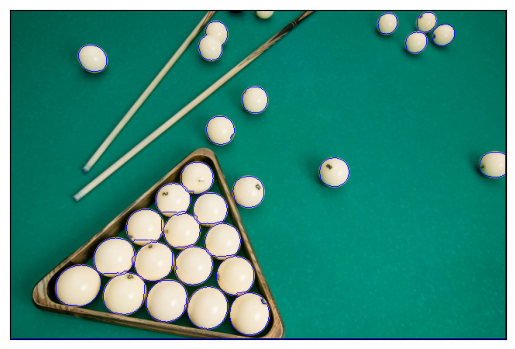
\includegraphics[width=0.4\textwidth]{result/3_result.png}
    \caption{Границы сегментов.}
\end{figure}

На итоговом изображении линии чётко разделяют соседние шары, несмотря на их касание.

Сделаем выводы:
\begin{itemize}
    \item Подход с дистанционной трансформацией и порогом 0.46·max даёт стабильные маркеры переднего плана даже при неоднородном освещении.
    \item Раздельное выявление фона через первую итерацию \texttt{watershed} помогает избежать ошибок алгоритма при касании объектов.
    \item Итеративное уточнение карты маркеров позволяет получить чёткие границы сегментов без значительных артефактов.
\end{itemize}

\section{Вывод}
В ходе выполнения лабораторной работы были достигнуты следующие результаты:
\begin{itemize}
  \item Исследованы и применены базовые морфологические операции (эрозия, дилатация, открытие, замыкание), благодаря чему удалось эффективно удалять внешние выступы и внутренние «дыры» на произвольном бинарном изображении, а также получать производные карты для анализа локальных дефектов.
  \item Реализован алгоритм поиска связных компонентов, что позволило маркировать отдельные объекты, вычислять их статистические характеристики и визуализировать каждую компоненту в отдельный цвет.
  \item На изображении с перекрывающимися объектами (игральные карты) разработана последовательность морфологических операций для выделения центральных «ядер», построения тонких разделительных линий и получения раздельных объектов путём побитовых масок и комбинирования результатов.
  \item Освоен метод (\texttt{watershed}) для сегментации касающихся круглых объектов (шары). Были выделены надёжные маркеры переднего и заднего планов через дистанционную трансформацию, порогирование и предварительный проход алгоритма, что позволило получить чёткие границы сегментов даже при их плотном соприкосновении.
\end{itemize}

В результате выполненной работы получены универсальные приёмы морфологической обработки, которые могут быть успешно применены в задачах фильтрации шумов, выделения контуров, разделения перекрывающихся объектов и подготовки данных для дальнейшего анализа.

\section{Вопросы к защите}
\begin{enumerate}
    \item \textbf{Включает ли результат открытия в себя результат закрытия?}\\[0.3em]
    Нет. Открытие (\(A\circ B = (A\ominus B)\oplus B\)) удаляет выступы и шум, а закрытие (\(A\bullet B = (A\oplus B)\ominus B\)) заполняет «дыры». Это разные операции с противоположными эффектами.

    \item \textbf{Какой морфологический фильтр необходимо применить, чтобы убрать у объекта выступы?}\\[0.3em]
    Операция \emph{открытия}: сначала эрозия для удаления выступов, затем дилатация для восстановления формы.

    \item \textbf{Каким образом с помощью морфологических операций можно найти контур объекта?} \\[0.3em]
    Контур можно получить как разницу между дилатацией и эрозией:  
    \[
      \mathrm{grad}(A,B) = (A\oplus B) - (A\ominus B).
    \]
    Для внутреннего контура: \(A - (A\ominus B)\), для внешнего: \((A\oplus B) - A\).
  

    \item \textbf{Что такое морфология?} \\[0.3em]
    Математическая морфология — раздел обработки изображений, изучающий преобразования множества пикселей с помощью структурного элемента для анализа и модификации формы объектов.
\end{enumerate}
\end{document}
